\chapter{OpenBTS based Cognitive Radio Test-Bed}

In this project we try to demonstrate the coexistence of \glspl{pu} and \glspl{su}
in the same \gls{gsm} frequency band by making the \glspl{su} switch to 
some neighboring unoccupied \gls{gsm} frequency band (spectrum hole) as soon as the 
\glspl{pu} of that frequency band makes a call. A spectrum hole is a 
frequency band/channel that have been licensed to the \glspl{pu} but is not 
being used at that particular space and time. This allows \glspl{su} to 
make use of already licensed frequency bands instead of having to allot them 
completely new frequency bands altogether.

In the first phase of the project, we implemented a 2-frequency system where
the secondary system had an option of switching into one of 2-frequency 
channels depending on which one was free. We expanded this to a 4-frequency
system with two primary systems in the second phase. The secondary would 
search for an unused frequency band among these four frequencies, two of which
always remain used.

\section{The 2-frequency system}
\subsection{Experimental setup of the 2-frequency system}

\begin{figure}
\centering
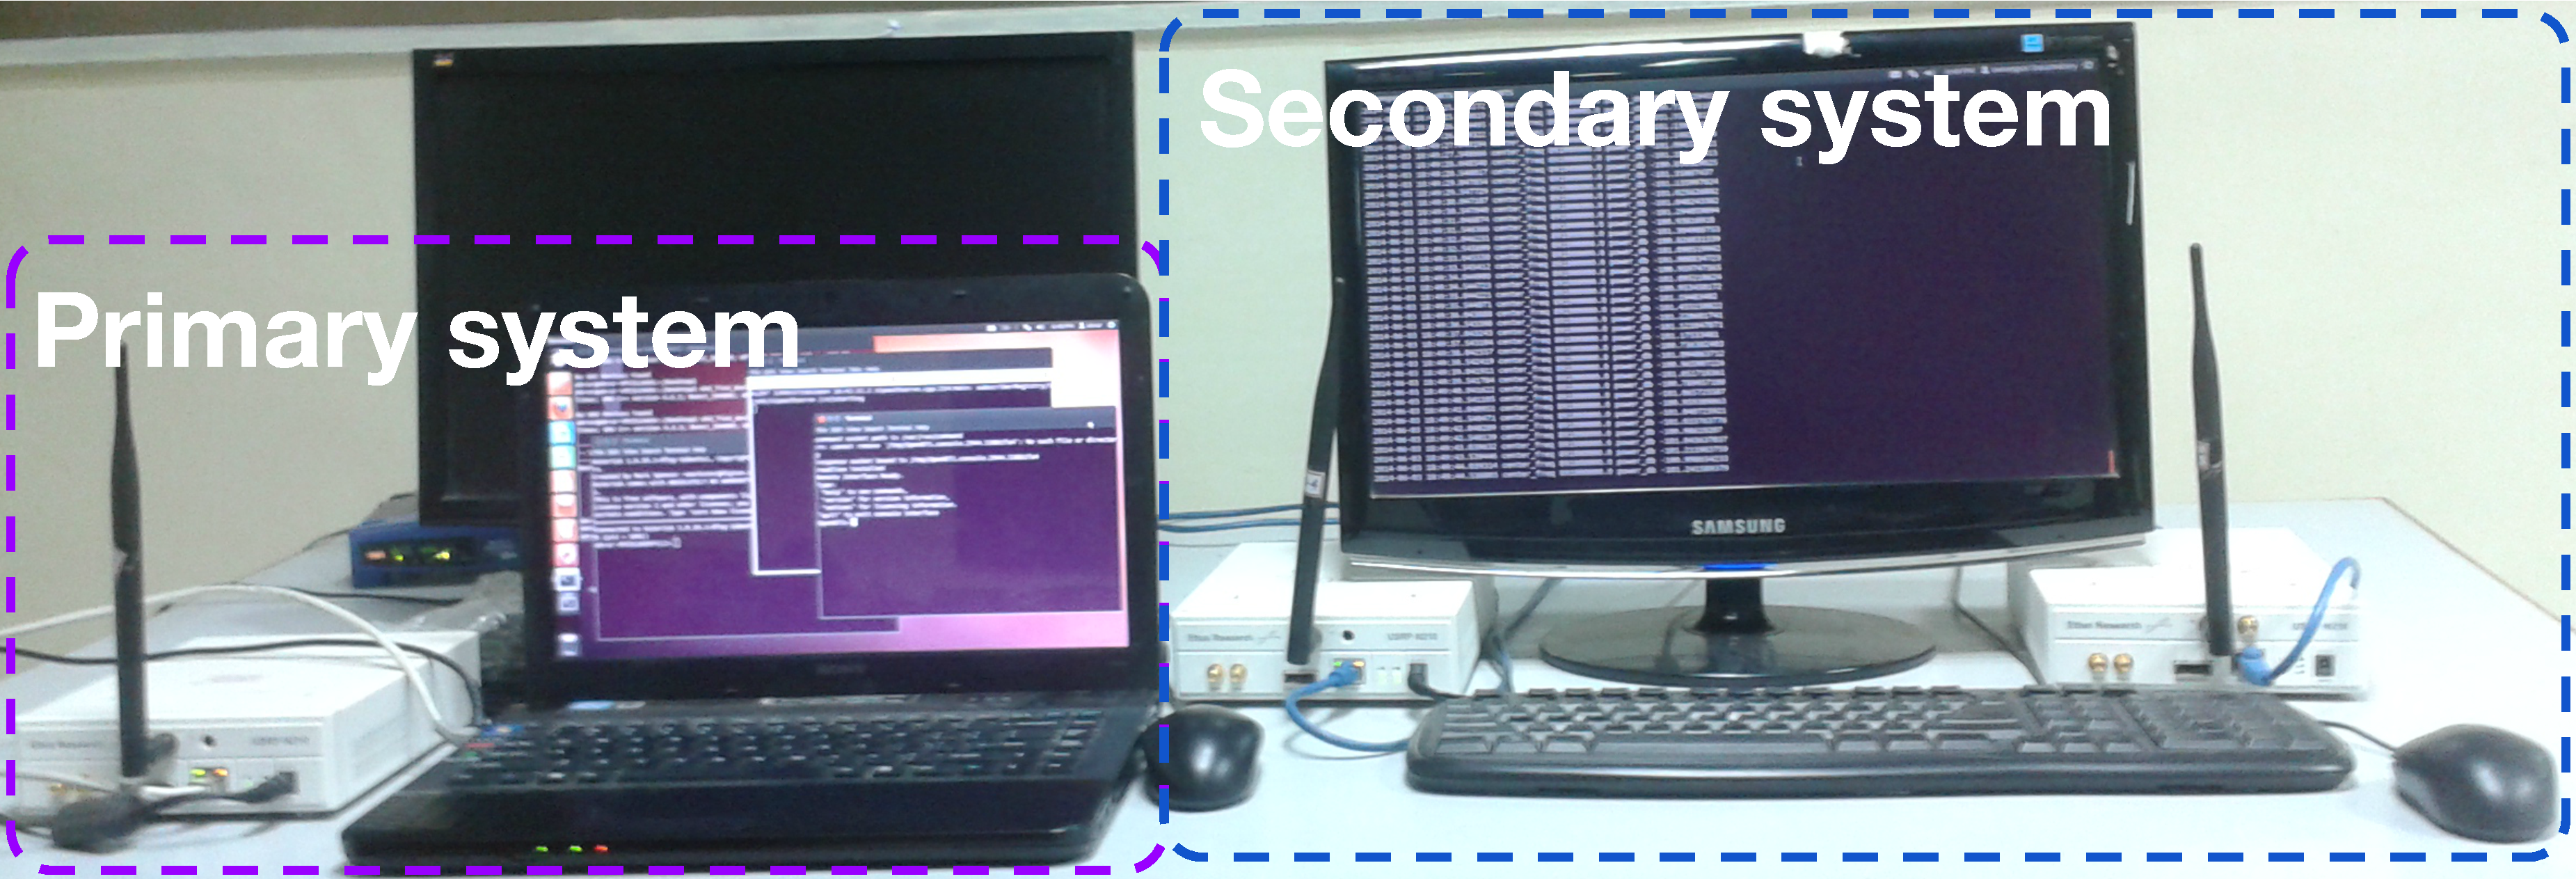
\includegraphics[width=1\textwidth]{../images/freq2}
\caption[Experimental setup, 2-frequency system]{Experimental setup of the 
2-frequency system}
\label{freq2}
\end{figure}



The hardware and software components used in this experiment are the 
following:
\begin{itemize}
    \item \textbf{A primary \gls{bts} --} This is a Linux laptop running OpenBTS
    software with 1 \gls{usrp} as the OpenBTS radio interface. The \gls{usrp} hardware kit
    has a WBX 50-2200 MHz RX/TX daughterboard in it. Two mobile phones 
    (\glspl{pu}) are connected to the OpenBTS network running in this 
    primary \gls{bts} system.
    \item \textbf{A secondary \gls{bts} --} This is an Ubuntu desktop running
    OpenBTS and GNURadio software. Two \gls{usrp} kits are connected to this
    machine, one as the OpenBTS radio interface and the other as the GNURadio
    radio interface. The GNURadio software is used for the spectrum sensing. 
    So, here the OpenBTS software with its radio interface acts as a \gls{bts}
    while the GNURadio software alongwith its radio
    interface acts as a spectrum sensor. Each of the two \gls{usrp} kits has a
    WBX 50-2200 MHz RX/TX daughterboard. Two other mobile phones (\glspl{su})
    are connected to the OpenBTS network running in this secondary \gls{bts}.
\end{itemize}

The secondary \gls{bts} system has cognitive capabilities. It was a challenge to 
make OpenBTS and GNURadio run simultaneously in the same computer and make 
them communicate with each other. GNURadio keeps sensing the spectrum used by
the \glspl{su} continuously in the background and takes decisions whether
to switch the frequency band of the secondary \gls{bts} or not, depending upon the 
energy level in the frequency band in which it is running.

\subsection{Testing of the 2-frequency system}
First we choose any two \gls{gsm} frequency bands say 945 MHz ($F_1$) and 950 MHz 
($F_2$). The \glspl{pu} are made to occupy $F_1$. Then we let the \glspl{su}
come into $F_1$. This makes the energy level in $F_1$ go high, which 
gets detected by the spectrum sensor of the secondary \gls{bts}. So, the secondary 
\gls{bts} moves out of $F_1$ and switches its frequency to $F_2$. Similarly, now if 
the \glspl{pu} are made to come into $F_2$, the secondary switches back to 
$F_1$.

In this experiment we don't have the situation where both $F_1$ and $F_2$ 
remain occupied because there is only one set of \glspl{pu}. Therefore, the 
secondary also doesn't check the energy level in a channel before taking the
decision to switch into that channel.

\begin{figure}
\centering
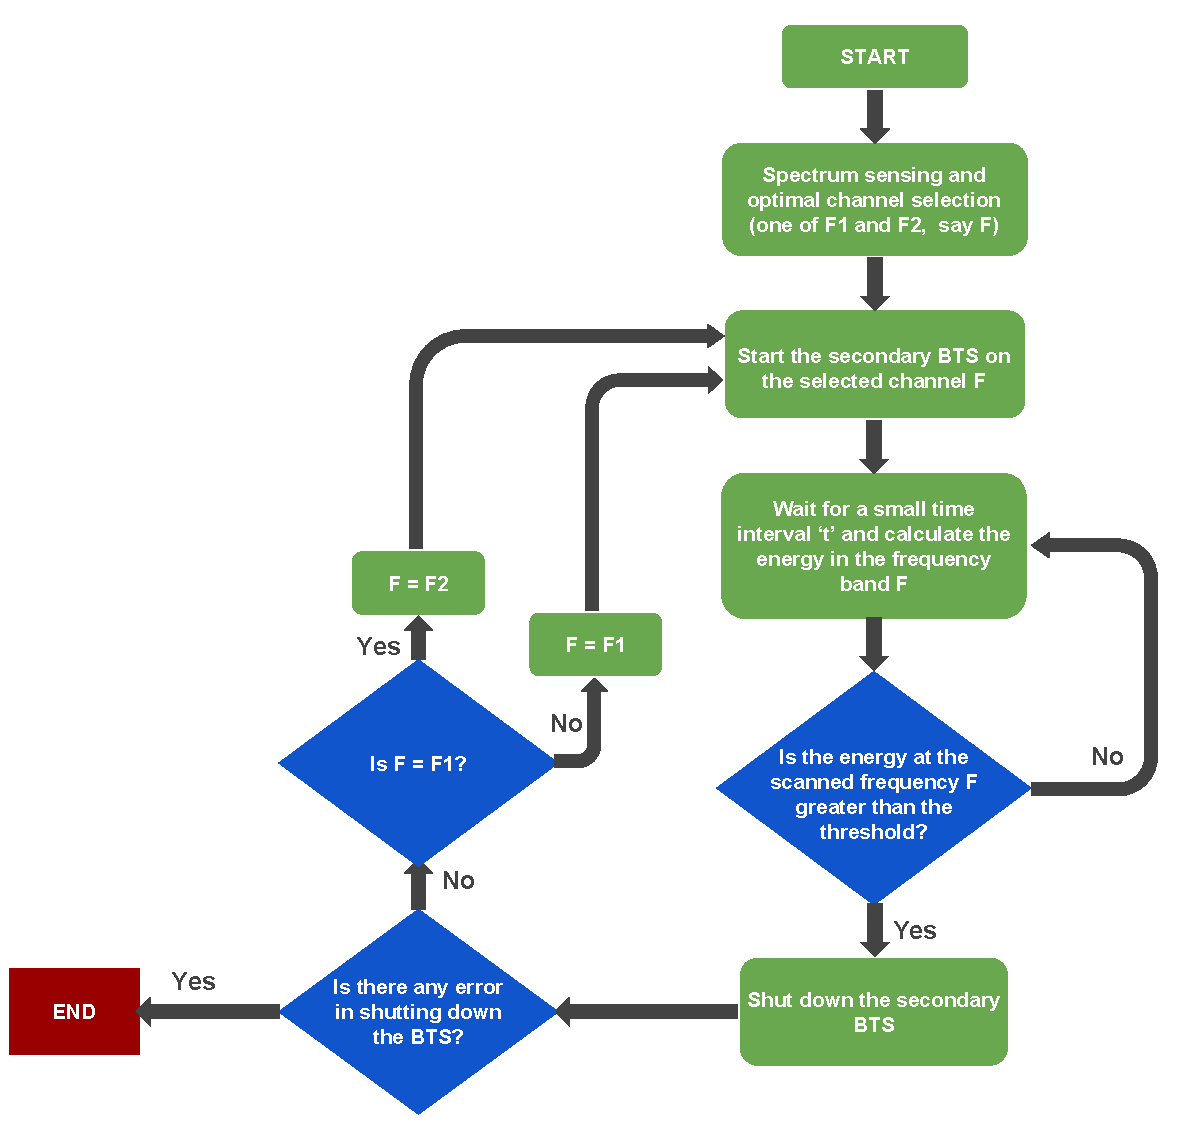
\includegraphics[width=1\textwidth]{../images/freqSys2}
\caption[2-frequency system]{Flowchart for the 2-frequency system}
\label{freqSys2}
\end{figure}



\section{The 4-frequency system}

As has been said earlier, in second phase, we expanded the 2-frequency
system to a 4-frequency one. The frequency channels are $F_1$ = 936 MHz, 
$F_2$ = 943 MHz, $F_3$ = 950 MHz, $F_4$ = 957 MHz. We also had two primary 
systems instead of just one this time. We also used a method known as CUSUM 
for peak detection in this case.

\begin{figure}
\centering
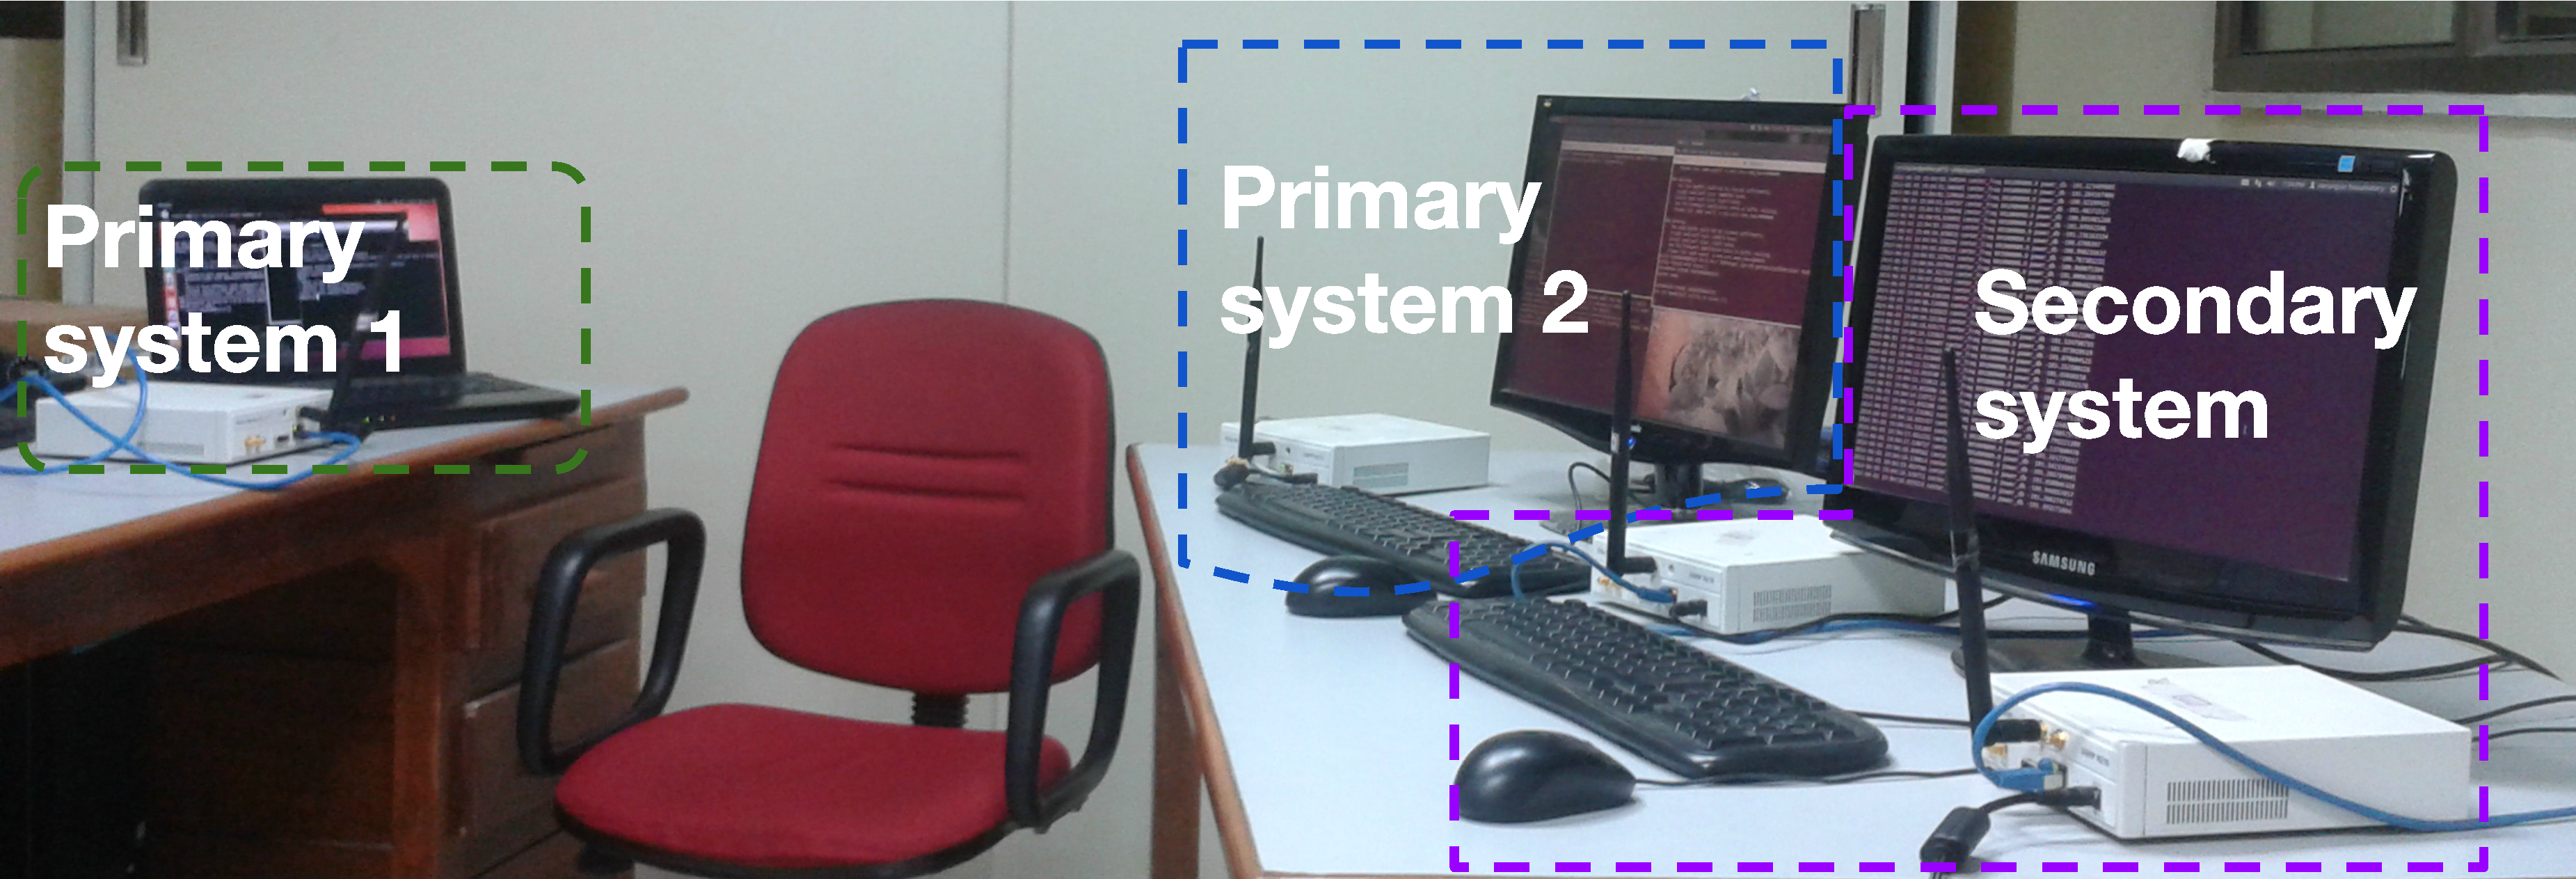
\includegraphics[width=1\textwidth]{../images/freq4}
\caption[Experimental setup, 4-frequency system]{Experimental setup of the 
4-frequency system}
\label{freq4}
\end{figure}

\subsection{Experimental setup of the 4-frequency system}
The tools used in this experiment are as follows:
\begin{itemize}
    \item \textbf{Two primary \glspl{bts} --} One is a laptop and the other one is a
    desktop. Both of them runs Ubuntu as the Operating System. Each one of
    them runs OpenBTS with a \gls{usrp} kit as its radio interface. A pair of mobile
    phones are connected to each one of them.
    \item \textbf{A secondary \gls{bts} --} This is the same as in the 
    2-frequency system. It runs OpenBTS and GNURadio on two different \gls{usrp}
    kits. A pair of mobile phones (\glspl{su}) are connected to its
    OpenBTS network.
\end{itemize}

One of the primary \glspl{bts} has a \gls{usrp} with a SBX 400-4400 MHz RX/TX 
daughterboard, the rest of the \glspl{usrp} all had a WBX daughterboard as before.

\subsection{Testing of the 4-frequency system}

Initially we make one of the primary systems operate in $F_2$. And the 
secondary is made to operate in $F_1$. Now we let the other primary come into 
$F_1$. The secondary senses it and attempts to switch to $F_2$ because the 
secondary is programmed to check $F_1$, $F_2$, $F_3$, $F_4$ serially in that 
order. After checking $F_4$ the secondary checks $F_1$, $F_2$, $F_3$, ... 
again and so on the cycle continues.

But the frequency $F_2$ happens to be occupied by the one of the primary 
systems. So, the secondary moves ahead to $F_3$ which is unoccupied and 
utilizes that channel.

Unlike the 2-frequency system, in this case the secondary always checks 
the availability of a channel before deciding to switch into it. In the 
2-frequency system, it was assumed that one of the two channels is always
unoccupied.

\begin{figure}
\centering
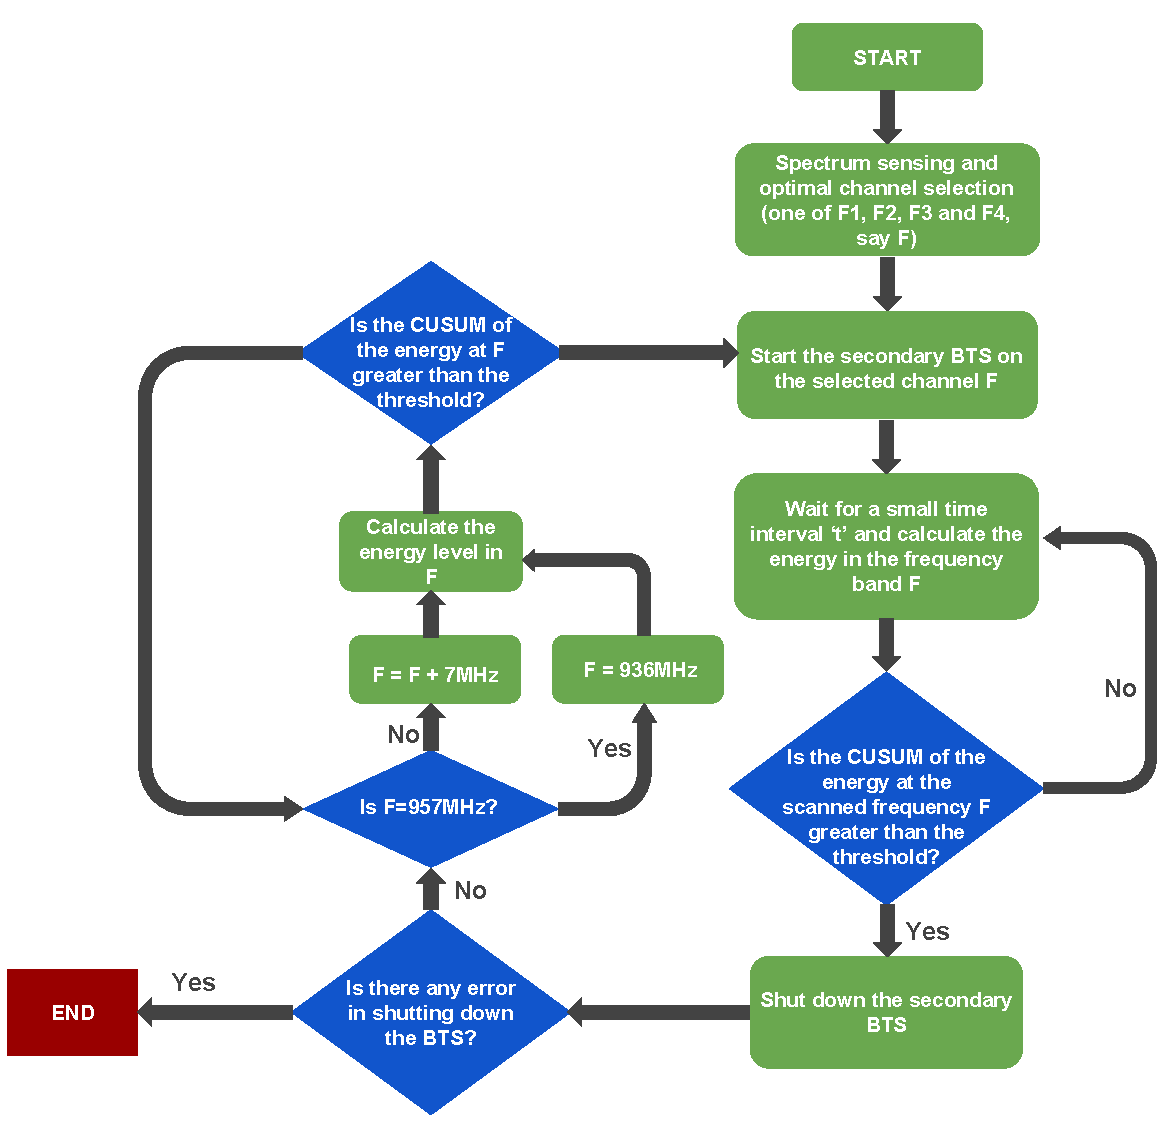
\includegraphics[width=1\textwidth]{../images/freqSys4}
\caption[4-frequency system]{Flowchart for  the 4-frequency system}
\label{freqSys4}
\end{figure}

The spectrum sensing is done using the energy detection based method. For 
making decisions whether to switch the frequency of the secondary \gls{bts} or not, 
a threshold of energy level is required to be set. If the energy level in a 
given channel is beyond the thresho ld, it implies that the \glspl{pu} are
also using that channel i.e. that channel is already occupied by \glspl{pu}

To choose a threshold energy level, we took various readings of the noise 
floor, energy when only \glspl{pu} were active, energy when only \glspl{su}
were active and also when both \glspl{pu} and \glspl{su} were 
active simultaneously for a short duration. The energy level threshold depends
on the distance of the mobile phones from the \gls{bts}. We can subdue this 
dependency on the distance by setting the threshold quite low so that even if
the users move farther away the decision making is not affected.

\section{CUSUM method}

The CUSUM (or cumulative sum control chart) method is used here to detect 
the peak in energy levels \cite{wikiCUSUM}. This method is used to ascertain 
that the peak in the energy levels in a given channel are not just due to some
irrelevant reasons like random fluctuations in the noise power, etc.
 
CUSUM is a technique used for monitoring change detection. It involves 
calculating the cumulative sum, which is what makes it sequential. The samples
from a process $x_n$ are assigned weights $\omega_n$ and summed in the 
following way:
\begin{align}
    S_0 &= 0 \nonumber \\
    S_n &= max(0, S_n + x_n - \omega_n) \nonumber
\end{align}

When the value of $S$ exceeds a certain threshold value, a change in value has 
been found. However, this formula detects only a change in the positive 
direction. For the negative direction, the $max$ operation has to be replaced 
by the $min$ operation. In this case the change has been found when the 
(negative) value is below the threshold value.


\section{Achievements}

What follows is a brief overview of the things done and the challenges faced 
during the course of the project.

\begin{enumerate}
    \item We began by trying to get acquainted with \gls{cr}. We 
    carried out a literature survey on \gls{cr} and also on the ongoing 
    research work in the field of \gls{cr}.
    \item Since GNURadio applications are written in the Python programming 
    language, we had to brush up our knowledge of the Python language.
    \item We familiarized ourselves with the GNURadio software package. Even 
    the installation procedure of GNURadio was a little challenging for us
    back then because GNURadio required a manual installation. We tweaked
    and played around with the already existing codes of signal processing
    blocks that come by default with GNURadio.
    \item We acquainted ourselves with the \gls{usrp} hardware kit, which happens to
    be the prime hardware used in our project. An outdoor experiment was
    carried out to estimate the range of the \gls{usrp} kit. This is largest 
    distance upto which mobile phones are able to get reasonable signal
    quality from the \gls{usrp}.
    \item Then we got familiar with the OpenBTS software. We had a hard time
    installing and configuring OpenBTS to work. But eventually we managed to 
    get our \glspl{sim} registered to the OpenBTS network and also to make calls and
    to text messages between the phones. The \gls{usrp} kit is the hardware radio 
    interface for the OpenBTS software.
    \item Spectrum sensing lies at the very heart of the entire operation of 
    \gls{cr}. So we surveyed literature on various methods of spectrum
    sensing. We made a decision to go with Energy detection based method 
    because it is comparatively less complicated and computationally less 
    resource-expensive. Average Periodogram Analysis is a technique used in 
    energy detection based spectrum sensing. So we carried out a study on
    Average Periodogram Analysis.
    \item After all these we prepared our problem statement and designed a 
    flow graph presenting our proposed algorithm to solve the problem. Then 
    we started developing the experimental setup that we have covered at the
    beginning part of this chapter.
    \item A key approach in solving our problem was to make GNURadio and 
    OpenBTS run simultaneously in the same computer hardware. This was a
    little tricky for us. Because we had to figure out if it was possible to
    run two \gls{usrp} kits on the same computer. Fortunately, it is possible if the
    two kits do not use the same IP address. So, we had to configure the kits
    to use different IP addresses. This was done by burning a different IP 
    address to one of the kits.
    \item Next we built a 2-frequency system which had a pair of \glspl{pu}
    and a pair of \glspl{su} communicating in parallel. The \glspl{pu} 
    were to be given higher priority. So the \glspl{su} would have
    to switch to a different and unoccupied channel as soon as the \glspl{pu}
    started making calls. A detailed description has already been given
    at the beginning part of this chapter.
    \item Then we extended the 2-frequency system to a 4-frequency system
    which has two pairs of \glspl{pu} instead of just one. Thus we have 
    demonstrated the coexistence of \glspl{pu} and \glspl{su} in the 
    same \gls{gsm} frequency band.
\end{enumerate}



